\documentclass[../DS04.tex]{subfiles}
\graphicspath{{./figures/}}

% \subimport{/home/nora/Documents/Enseignement/Prepa/bpep/exercices/DS/resonance_verre/}{sujet.tex}

\begin{document}

\section[50]"P"{Résonance d'un verre\ifcorrige{~\small\textit{(D'après TSI Centrale
		Supélec 2018)}}}

\enonce{%
Dans le vingt-et-unième album de la série {\it Les Aventures de Tintin},
intitulé {\it Les Bijoux de la Castafiore}, cette dernière est en mesure de
faire exploser un verre par la simple utilisation de sa voix. Le présent sujet
se penche sur les aspects physiques de ce phénomène. Nous tenterons ainsi de
déterminer les circonstances dans lesquelles il est effectivement possible de
réaliser une telle prouesse et nous nous pencherons sur les rôles joués par les
différents paramètres physiques susceptibles d'influer sur ces circonstances.
}

\partie{Analyse expérimentale des vibrations du verre suite à un choc}

\enonce{%
	Il est extrêmement facile, en frappant un verre à pied, d'entendre le son que
	celui-ci émet. On se propose dans cette partie de déterminer, à partir d'une
	modélisation simple, quelques propriétés des oscillations libres d'un verre
	mis ainsi en vibration.
	\begin{center}
		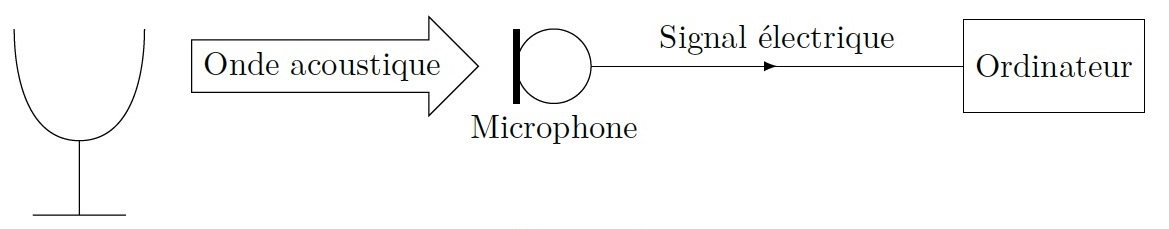
\includegraphics[width=.6\linewidth]{res_verre_1}
		\captionof{figure}{Schéma de principe.}
		\label{fig:schema_principe}
	\end{center}

	Un verre à pied, d'un diamètre de \SI{12}{cm}, est frappé, à l'instant $t=0$,
	au niveau du bord supérieur à l'aide d'un petit marteau. Le son émis est
	enregistré par ordinateur et représenté sur la figure \ref{fig:chronogramme}.
	Le spectre de ce signal temporel est représenté sur la figure
	\ref{fig:spectre}.
	\smallbreak
	\noindent
	\begin{minipage}[c]{.42\linewidth}
		\begin{center}
			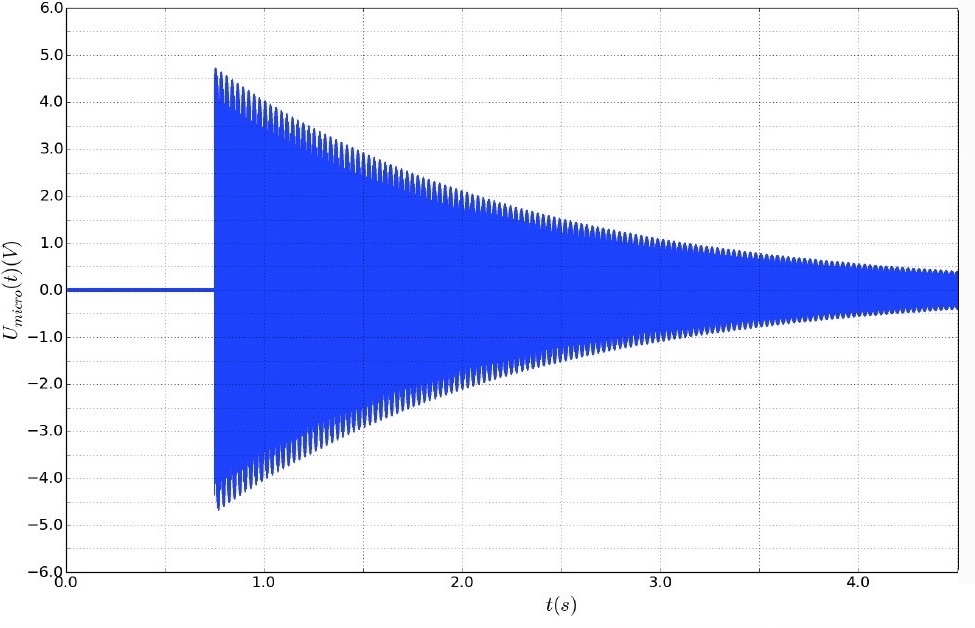
\includegraphics[width=\linewidth]{res_verre_2}
			\captionof{figure}{Chronogramme de l'enregistrement sonore du verre.}
			\label{fig:chronogramme}
		\end{center}
	\end{minipage}
	\hfill
	\begin{minipage}[c]{.5\linewidth}
		\begin{center}
			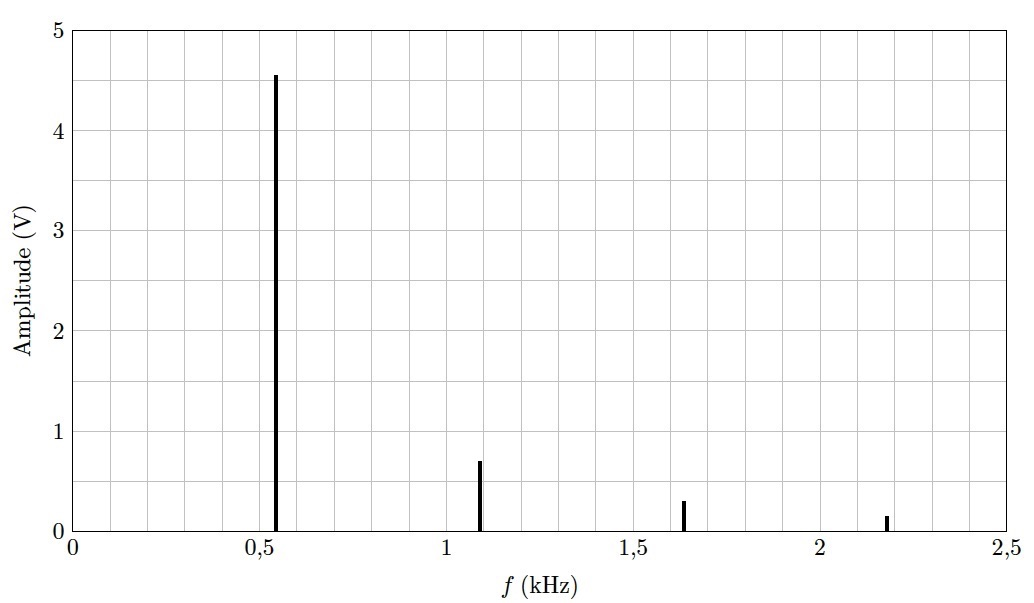
\includegraphics[width=\linewidth]{res_verre_3}
			\captionof{figure}{Analyse spectrale du son réalisé peu après la frappe du
				verre.}
			\label{fig:spectre}
		\end{center}
	\end{minipage}
	\bigbreak
	Les «~pics~» représentés dans la figure \ref{fig:spectre} correspondent à des
	modes propres de vibration du verre.
}

\QR{%
	Donner les fréquences des différents modes propres. Elles sont liées par une
	relation simple, laquelle~?
}{%
	On relève les fréquences suivantes : $f_1\approx \SI{550}{Hz}$, $f_2\approx
		\SI{1090}{Hz}$, $f_3\approx \SI{1620}{Hz}$ et $f_4\approx \SI{2180}{Hz}$. On
	remarque donc que l'on a $\boxed{f_n= n f_1}$, avec $n\in \mathbb{N}^*$
}

\QR{%
	Comment nomme-t-on ces différents modes propres ?
}{%
	Le premier mode est appelé \xul{fondamental}. Les autres sont appelés
	\xul{harmoniques de rang $n$}.
}

\QR{%
	Quelle est la fréquence du signal~?
}{%
	La fréquence du signal est la fréquence de son fondamental, donc ici
	\xul{$f=\SI{550}{Hz}$.}
}

% \QR{%
%   À l'aide d'un modèle simple, que vous exposerez clairement, déterminer la
%   vitesse de propagation de l'onde de choc dans le verre. \textit{Cette question
%   nécessite de prendre des initiatives. Il n'est pas nécessaire d'y avoir
% répondu pour poursuivre le problème. La notation portera sur l'ensemble de la
% démarche mise en place (identification des phénomènes physiques intervenant,
% hypothèses simplificatrices, etc) et non pas sur le seul résultat.}
% }{%
%   La présence de plusieurs modes propre indique qu'on est en présence d'ondes
%   stationnaires de même type que celles de la corde de \bsc{Melde}.
%
%   Or, le mode fondamental de la corde de \bsc{Melde} se caractérise par une
%   fréquence fondamentale $f_0=\frac{c}{\lambda}$ avec $\lambda=2L$. La longueur
%   d'onde est donc égale à la distance parcourue par l'onde pour revenir au point
%   où elle a été émise. En effet, on peut aussi voir le problème en terme
%   d'interférences : quand l'onde réfléchie atteint le vibreur, elle a parcourue
%   une longueur d'onde et se trouve donc en phase avec l'onde émise par le
%   vibreur, ce qui crée des interférences constructives entre les deux ondes, et
%   donc un mode de résonance.
%
%   Dans le cas de l'onde de choc se propageant dans le verre, on peut considérer,
%   pour simplifier le problème ici que l'onde se propage en suivant le bord du
%   verre. Sur le même principe que la corde de \bsc{Melde}, la longueur d'onde du
%   mode fondamental doit donc être égale à la distance parcourue par l'onde avant
%   de revenir à son point de départ, soit $\lambda=2\pi R=\pi D$. On a alors
%   $c=\lambda f$. L'application numérique donne $c=\pi \times 0,12 \times 540
%   \approx \SI{2,0e2}{m.s^{-1}}$.
% }

\vspace{0.5cm}
\enonce{%
	Quand le verre est en vibration, son bord supérieur oscille autour de sa
	position au repos. Afin d'estimer le facteur de qualité du verre, on le
	modélise par une masse $m$ mobile sur l'axe $(Ox)$ horizontal associée à un
	ressort de raideur $k$, de longueur à vide nulle (figure
	\ref{fig:schema_mecanique_verre}). Les frottements seront, quant à eux,
	modélisés par un frottement fluide de type $\vec f = - \alpha \vec v$ où $\vec
		v$ désigne le vecteur vitesse
	de la masse $m$.
}

\begin{center}
	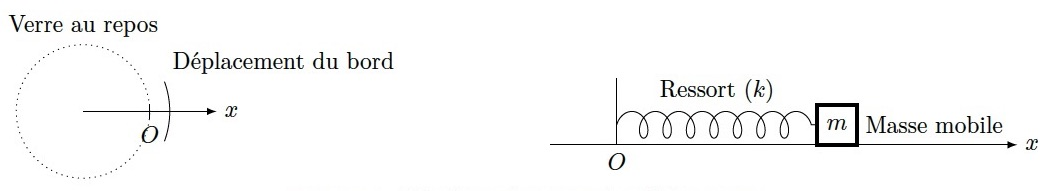
\includegraphics[width=.8\linewidth]{res_verre_4}
	\captionof{figure}{Modèle mécanique du déplacement.}
	\label{fig:schema_mecanique_verre}
\end{center}

% \figCap{0.8}{res_verre_4.jpg}{\protect\label{fig:schema_mecanique_verre} }

\QR{%
Montrer que l'équation différentielle traduisant l'évolution temporelle de $x(t)$ s'écrit de la façon suivante, avec $\w_0$ et $Q_0$ deux constantes que l'on exprimera en fonction de  $\alpha$, $k$ et $m$ :
\eq{
\dv[2]{x}{t} + {\frac{\w_0}{Q_0}}{\dv{x}{t}} + \w_0^2 x = 0
}

\textit{On portera une attention particulière à la rédaction de cette question.}
}{%
On étudie le point $M$ dans le référentiel terrestre supposé galiléen.

Bilan des forces :
\begin{itemize}
	\item Poids $\vec{P}=-mg\vec{u}_z$ où $\vec{u}_z$ désigne la verticale ascendante
	\item Réaction du support $\vec{R}=R\vec{u}_z$
	\item Force de rappel élastique $\vec{F}=-kl\vec{u}_x=-kx\vec{u}_x$ car $l_0=0$
	\item Force de frottement $\vec{f}=-\alpha\vec{v}=-\alpha\dot{x}\vec{u}_x$
\end{itemize}
D'après le principe fondamental de la dynamique, on a
\eq{
	m\vec{a}=\vec{P}+\vec{R}+\vec{F}+\vec{f}
}

avec $\overrightarrow{OM}=x\vec{u}_x$, donc $\vec{v}=\dot{x}\vec{u}_x$, donc $\vec{a}=\ddot{x}\vec{u}_x$

Ainsi, en projetant cette relation sur $Ox$ on a
\eq{
	m\ddot{x}=-\alpha x-kx\Leftrightarrow \boxed{\ddot{x}+\frac{\alpha}{m}\dot{x}+\frac{k}{m}\dot{x}=0}
}

On obtient bien la forme demandée avec $\boxed{\w_0=\sqrt{\dfrac{k}{m}}}$ et $\dfrac{\w_0}{Q_0}=\dfrac{\alpha}{m} \Leftrightarrow\boxed{ Q_0=\frac{1}{\alpha}\sqrt{km}}$
}


\QR{%
	Quelle est la signification physique de $\w_0$ et de $Q_0$ ? Quelles sont les unités de ces deux grandeurs ?
}{%
	$\w_0$ est la pulsation propre du systèmen elle s'exprime en \si{rad/s}. Elle correspond à la pulsation à laquelle oscillerait le système s'il n'y avait pas de frottement.

	$Q_0$ est appelé facteur de qualité du système. Il est sans unité. Plus $Q_0$ est grand, moins il y a de dissipation d'énergie, plus le système s'approche d'un oscillateur harmonique non amorti.
}


\QR{%
Compte tenu du choc initial avec le marteau, déterminer, dans le cas d'un frottement \og faible \fg, l'expression approchée de la solution $x(t)$ avec les conditions initiales $x(0) = 0$ et $\dv{x}{t}(0) = V_0$. Montrer en particulier que la fonction $x(t)$ peut se mettre sous la forme d'un signal sinusoïdal de pulsation $\w$ délimité par une enveloppe exponentielle décroissante, dont on précisera l'expression du temps caractéristique $\tau$ en fonction de $\w_0$ et $Q_0$.
}{%
L'équation différentielle est homogène, donc $x(t)=x_h(t)$. Pour déterminer $x_h(t)$, on cherche les racines de l'équation caractéristique
\eq{
	r^2+\frac{\w_0}{Q_0} r+\w_0^2=0
}

On calcule donc son discriminant : $\Delta =\pa{\frac{\w_0}{Q_0}}^2-4\w_0^2=\frac{\w_0^2}{Q_0^2}(1-4Q_0^2)$

Dans le cas d'un frottement \og faible \fg, $Q_0$ est \og grand\fg. On peut donc supposer que $\Delta <0$. On se trouve alors en régime pseudo-périodique. Les solutions de l'équation caractéristique sont donc :
\eq{
	r=-\frac{\w_0}{2Q_0}\pm j\frac{\w_0}{2Q_0}\sqrt{4Q_0^2-1}= -\frac{1}{\tau} \pm j\W
}

avec $ \boxed{\tau=\frac{2Q_0}{\w_0}}$ et $\boxed{\W=\frac{\w_0}{2Q_0}\sqrt{4Q_0^2-1}}$

Ainsi, on a
\eq{
x(t)=e^{-\frac{t}{\tau}}(A\cos(\W t)+B\sin(\W t))
}

A $t=0$, on a $\boxed{x(0)=A=0}$.

Ainsi $\dot{x}=-\frac{1}{\tau }e^{-\frac{t}{\tau}}B\sin(\W t)+e^{-\frac{t}{\tau}} B\W\cos(\w t)$

A $t=0$, $\dot{x}(0)=B\W=V_0 \Leftarrow \boxed{B=\frac{V_0}{\W}}$

Finalement,
\eq{
\boxed{x(t)=e^{-\frac{t}{\tau}}\dfrac{V_0}{\W}\sin(\W t)}
}

}


\QR{%
	A l'aide de la figure \ref{fig:chronogramme}, déterminer numériquement $\tau$. \textit{On pourra faire apparaître les relevés ou constructions graphiques utilisés sur la copie de la figure \ref{fig:chronogramme} fournie en annexe.}
}{%
	\begin{center}
		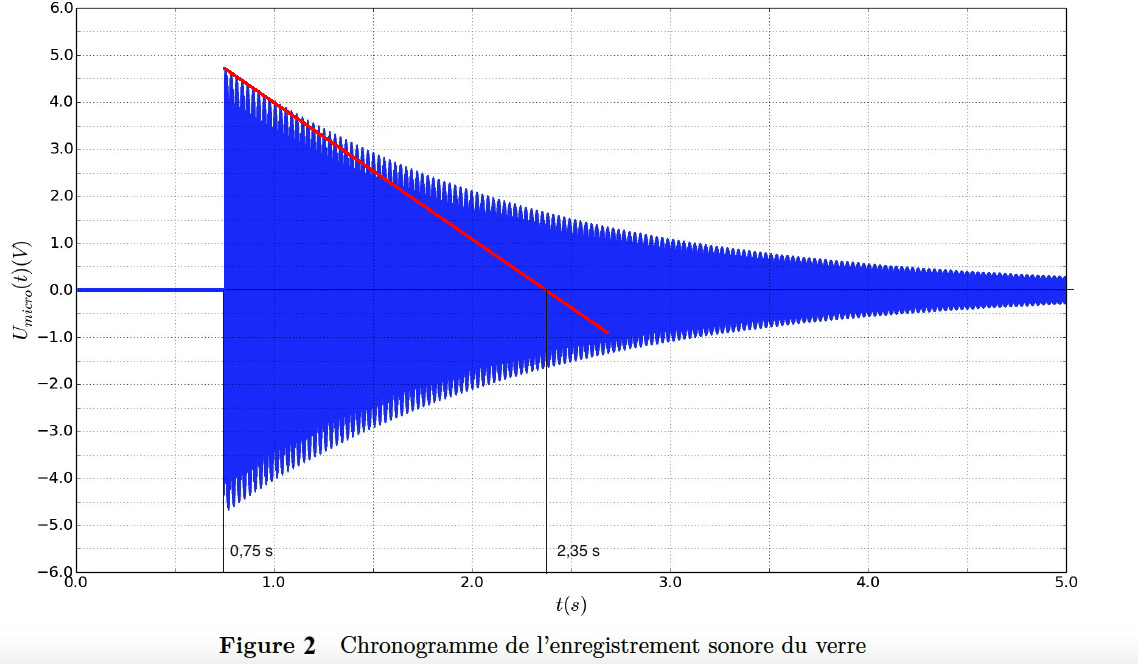
\includegraphics[width=.6\linewidth]{res_verre_2c}
	\end{center}

	On trace la tangente à l'origine de l'enveloppe exponentielle. Elle coupe l'asymptote $x=0$ en $t=\tau$. On lit donc \xul{$\tau\approx 2,35-0,75=1,6$ s}. En effet, sur le graphique, l'excitation a lieu à $t=0,75$ s et non $t=0$ comme dans la résolution mathématique.
}


\QR{%
	Comment se simplifie l'expression de la pseudo-pulsation $\w$ avec l'hypothèse des faibles frottements (justifier précisément) ?
}{%
	On a déjà vu lors de la résolution de l'équation que $\boxed{\W=\frac{\w_0}{2Q_0}\sqrt{4Q_0^2-1}}$

	On remarque que de très nombreuses pseudo-périodes sont visibles, on a donc
	$Q_0\gg 1$. Ainsi, $\W\approx \frac{\w_0}{2Q_0}\sqrt{4Q_0^2-\cancel{1}}$, soit
	$\boxed{\W\approx\w_0}$.
}


\QR{%
	Déduire des questions précédentes les valeurs numériques de $\w_0$ et $Q_0$.
	Commenter le résultat.
}{%
	On a relevé précédemment la fréquence du signal $f=\SI{550}{Hz}$, Comme on a
	montré que $\W\approx \w_0$, on en déduit \xul{$\w_0=2\pi f_0\approx
			\SI{3,5e3}{ rad/s}$}.

	Par ailleurs, $\tau=\frac{2Q_0}{\w_0} \Leftrightarrow Q_0=\frac{\w_0
			\tau}{2}=\pi f_0 \tau$. L'application numérique donne \xul{$Q_0\approx
			2,8.10^3$}.
}

\partie{Étude de la résonance en amplitude du verre en régime sinusoïdal forcé}

\enonce{
On souhaite étudier plus finement la réponse en amplitude du verre au voisinage de la fréquence de résonance du mode 1 précédemment déterminée.

Un haut-parleur relié à un générateur basse fréquence produit une onde sonore sinusoïdale de fréquence $f$. Le verre, placé à proximité du haut-parleur (figure \ref{fig:excitation_verre}), est ainsi placé en régime
sinusoïdal forcé.

\begin{center}
	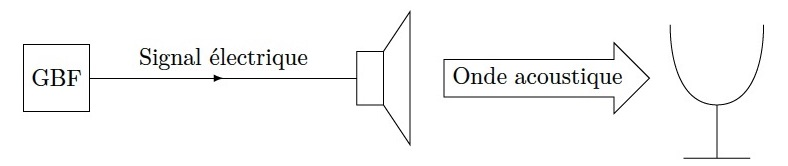
\includegraphics[width=.5\linewidth]{res_verre_5}
	\captionof{figure}{}
	\label{fig:excitation_verre}
\end{center}

% \figCap{0.5}{res_verre_5.jpg}{\protect\label{fig:excitation_verre}}

L'équation différentielle traduisant l'évolution temporelle de $x(t)$ est alors de la forme suivante, avec $\w = 2\pi f$ la pulsation et $\Phi$ la phase du signal acoustique délivré par le générateur basse fréquence :
\eq{
\dv[2]{x}{t} + {\frac{\w_0}{Q_0}} \dv{x}{t} + \w_0^2 x= A_0 \cos(\w t + \Phi)
}

En régime sinusoïdal forcé, la solution est de la forme $x(t) = X\cos(\w t + \varphi)$. On introduit la grandeur complexe associée $\xu(t) = \Xu \exp(\jw t)$ avec $j^2 = -1$.
}


\QR{%
Comment nomme-t-on la grandeur $\Xu$ ? Que représente son module, son
argument~?
}{%
$\Xu$ est appelée \xul{amplitude complexe} associée à $x(t)$.
$\Xu=Xe^{j\varphi}$, on a donc $\boxed{\abs{\Xu}=X}$ et $\boxed{\arg{\Xu}=\varphi}$.
}


\QR{%
Établir l'expression du module de $\Xu$ en fonction de $\w$, $\w_0$, $A_0$, $\Phi$ et $Q_0$.
}{%
On réécrit l'équation différentielle en mode fréquentiel :
\eq{
(j\w)^2 \Xu+\frac{\w_0}{Q_0}j\w \Xu+\w_0^2\Xu=\xul{A}=A_0e^{j\Phi}
}

On en déduit ensuite :
\eq{
\Xu=\frac{A_0e^{j\Phi}}{\w_0^2-\w^2+j\w\frac{\w_0}{Q_0}}
\Rightarrow \boxed{\Xu=\frac{A_0e^{j\Phi}/\w_0^2}{1-\pa{\frac{\w}{\w_0}}^2+j\frac{1}{Q_0}\frac{\w}{\w_0}}} \\
\Rightarrow \abs{\Xu} = \frac{A_0/\w_0^2}{\sqrt(1-u^2)^2+(u/Q_0)^2}
}

avec $u=\w / \w_0$. (on note $u$ car la variable $x$ est déjà utilisée !).
}


\QR{%
À partir d'une étude qualitative mais précise, justifier le numéro de graphe de
la figure \ref{fig:bodes} compatible avec le tracé du module de $\Xu$ en
fonction de la pulsation $\w$.
}{%
On fait une étude en hautes et basses fréquences~:

$\bullet$ En BF, $\w\ll \w_0$, on a donc
\eq{
\Xu=\frac{A_0e^{j\Phi}/\w_0^2}{1-\cancel{\pa{\frac{\w}{\w_0}}^2}+\cancel{j\frac{1}{Q_0}\frac{\w}{\w_0}}}\sim \frac{A_0e^{j\Phi}}{\w_0^2}
}

On a donc $\boxed{X \Sim_{\w \ll \w_0} \frac{A_0}{\w_0^2}}$

On a donc une asymptote horizontale en BF.

$\bullet$ En HF, $\w\gg \w_0$, on a donc
\eq{
\Xu=\frac{A_0e^{j\Phi}/\w_0^2}{\cancel{1}-\pa{\frac{\w}{\w_0}}^2+\cancel{j\frac{1}{Q_0}\frac{\w}{\w_0}}}\sim \frac{A_0e^{j\Phi}}{\w^2}
}

On a donc  $\boxed{X \Sim_{\w \gg \w_0} \frac{A_0}{\w^2}\propto \frac{1}{\w^2}}$

La courbe doit tendre vers zero en HF.

On en déduit donc qu'il s'agit du \xul{graphe 2}.
}

\enonce{%
	\begin{center}
		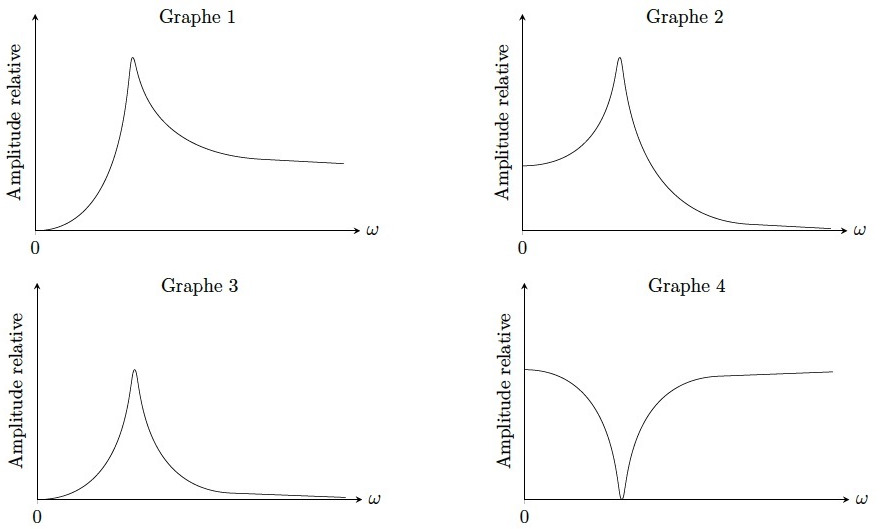
\includegraphics[width=0.7\linewidth]{res_verre_6}
		\captionof{figure}{Module de $\Xu$ en fonction de $\w$.}
		\label{fig:bodes}
	\end{center}
	% \figCap{0.7}{res_verre_6.png}{\protect\label{fig:bodes} }
}


\QR{%
Montrer qu'il ne peut y avoir de résonance que si $Q_0>Q_{lim}$ et déterminer
$Q_{lim}$.
}{%
Pour la suite de la question, on pose $u=\frac{\w}{\w_0}$ pour alléger les
calculs. Pour qu'il y ait résonance, il faut que $\abs{\Xu}=X$ passe par un
maximum pour $u\neq 0$. Or,
\eq{
	X=\frac{A_0/\w_0^2}{\sqrt{(1-u^2)^2+\frac{u^2}{Q_0^2}}}
}

Le numérateur est constant et la fonction racine carrée monotone donc $X$ passe
par un maximum si la fonction $f(u)=(1-u^2)^2+\frac{u^2}{Q_0^2}$ passe par un
minimum. On cherche donc l'annulation de la dérivée de $f(u)$.
\eq{
	\dv{f}{u}=2(-2u)(1-u^2)+\frac{2u}{Q_0}=-4u(1-u^2)+\frac{2u}{Q_0^2}
}

Ainsi,
\eq{
	\dv{f}{u}=0\Leftrightarrow -4u(1-u^2)+\frac{2u}{Q_0^2}=0
	\Leftrightarrow -2(1-u^2)+\frac{1}{Q_0^2}=0\text{ ou}u=0
}

La solution $u=0$ n'est pas acceptable car c'est une limite (limite BF)

On doit donc avoir
\eq{
	2(1-u^2)=\frac{1}{Q_0^2}\Leftrightarrow 1-u^2=\frac{1}{2Q_0^2}\Leftrightarrow u^2=1-\frac{1}{2Q_0^2}
}

Cette équation ne possède de solution que si $1-\frac{1}{2Q_0^2}>0\Leftrightarrow \boxed{Q_0>\frac{1}{\sqrt{2}}}$.

On en déduit donc $\boxed{Q_{lim}=\frac{1}{\sqrt{2}}}$
}


\QR{%
	Dans le cas d'une résonance, exprimer la pulsation correspondante, notée
	$\w_r$ en fonction de $\w_0$ et $Q_0$.
}{%
	Dans le cas précédent, $f'(u)$ s'annule pour $u_r=\sqrt{1-\frac{1}{2Q_0^2}}$,
	soit $\boxed{\w_r=\w_0 \sqrt{1-\frac{1}{2Q_0^2}}}$. Cette pulsation est celle
	qui maximise $X$, c'est donc la pulsation de résonance.
}

\enonce{%
	Dans la suite, on suppose $Q_0 \gg Q_{lim}$.
}

\QR{%
	Comment se simplifie alors l'expression de la pulsation de résonance $\w_r$ ?
}{%
	Si $Q_0\gg Q_{lim}$, alors $Q_0\gg 1$, et on a $\boxed{\w_r=\w_0
			\sqrt{1-\cancel{\dfrac{1}{2Q_0^2}}}\approx \w_0}$
}

\QR{%
	On note $X_r$ le module de $\Xu$ pour $\w =\w_r$. Établir son expression en
	fonction de $\w_0$, $A_0$ et $Q_0$.
}{%
	Par définition $X_r=X(\w_r)$. D'après la question précédente, on a donc
	$X_r\approx X(\w_0)=X(u=1)$, ce qui donne
	$X_r=\dfrac{A_0/\w_0^2}{\sqrt{\frac{1}{Q_0^2}}}\Leftrightarrow
		\boxed{X_r=Q_0\dfrac{A_0}{\w_0^2}}$
}

\QR{%
	Quelles sont les définitions des pulsations de coupure $\w_1$ et $\w_2$ ($\w_1
		< \w_2$) du module de $\Xu$ ? On ne cherchera pas ici à établir leurs
	expressions.
}{%
	Les pulsations de coupures sont définies par
	$\boxed{\abs{\Xu}(\w_1)=\abs{\Xu}(\w_2)=\frac{X_r}{\sqrt{2}}}$
}

\QR{%
	Quelle relation existe-t-il entre $\w_0$,~$Q_0$ et $\Delta\w = \w_2 - \w_1$ ? \textit{On admettra que cette relation est la même que dans le cas d'une résonance de type \og passe-bande \fg.}
}{%
	L'acuité de la résonance est égale à $Q_0$, soit $\boxed{\dfrac{\w_0}{\Delta \w}=Q_0}$
}

\enonce{
	Une série de mesures de l'amplitude $X$ au voisinage de la résonance (réalisée par un dispositif interférentiel non présenté ici) permet de tracer le graphe représenté sur la figure \ref{fig:bode_expe}.
}

\begin{center}
	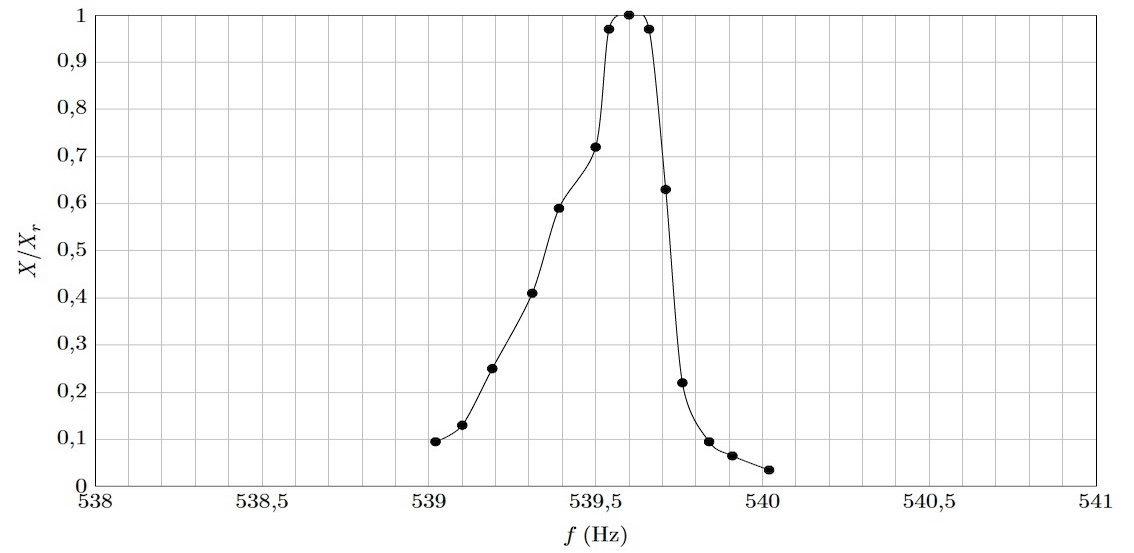
\includegraphics[width=.75\linewidth]{res_verre_7}
	\captionof{figure}{Amplitude relative en fonction de la fréquence.}
	\label{fig:bode_expe}
\end{center}

% \figCap{0.75}{res_verre_7.jpg}{\protect\label{fig:bode_expe} }

\QR{%
	Déterminer, à l'aide de la figure \ref{fig:bode_expe}, la pulsation propre $\w_0$ et le facteur de qualité $Q_0$ du verre dans son mode 1.  \textit{On pourra faire apparaître les relevés ou constructions graphiques utilisés sur la copie de la figure \ref{fig:bode_expe} fournie en annexe.}Comparer avec les résultats de la première partie.
}{%
	\begin{center}
		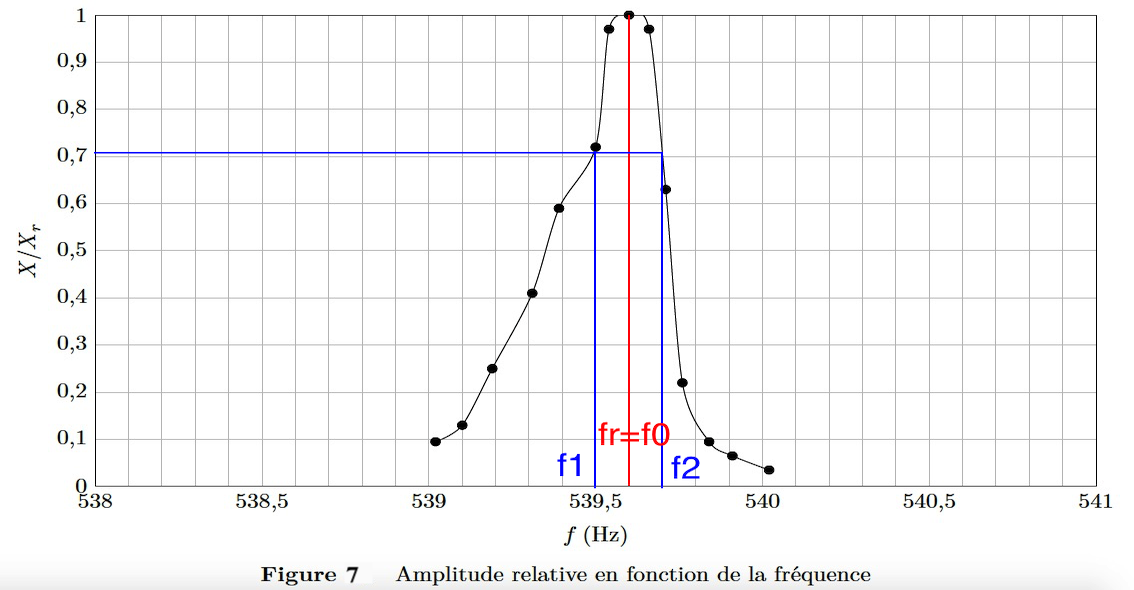
\includegraphics[width=.7\linewidth]{res_verre_7c}
	\end{center}

	% \fig{0.7}{res_verre_7c.png}


	On a vu précédemment que le système étudié possédait bien un facteur de qualité très élevé, on a donc $\w_r\approx \w_0$. On relève $f_r=f_0=\SI{539,6}{Hz}$, soit \xul{$\w_0=\SI{3390}{rad.s^{-1}}$}.

	Les fréquences de coupures valent respectivement $f_1=\SI{539,5}{Hz}$ et $f_2=\SI{539,7}{Hz}$ telles que $X/X_r=\frac{1}{\sqrt{2}}\approx 0,71$.

	On en déduit $Q_0= \dfrac{\w_0}{\w_2 - \w_1} = \dfrac{f_0}{f_2-f_1}=2,7.10^3$.

	On retrouve bien environ les mêmes valeurs que dans la première partie. La
	détermination de $\w_0$ est cependant plus précise au vu de l'échelle du
	graphique.
}


\QR{%
	En musique, la gamme tempérée comporte 12 demi-tons (do - do$\#$ - ré - ré$\#$ - mi - fa - fa$\#$ - sol - sol$\#$ - la - la$\#$ - si). Pour passer d'une note à la note suivante, on multiplie sa fréquence par $2^{1/12}$. Sachant que le la4 se trouve à 440 Hz, quelle note doit chanter la Castafiore pour briser le verre ? Chante-elle juste ?
}{%
	Pour briser le verre, il faut le mettre en résonance de sorte à ce qu'il vibre avec une amplitude telle que la déformation du matériau provoque sa rupture. Il faut donc l'exciter à la fréquence de 540 Hz.

	Si on a la note la à 440 Hz, alors les notes suivantes dans la gamme ont pour fréquences : 466 Hz (la$\#$) (si), 493 Hz (do), 523 Hz (do$\#$) et 554 Hz (ré).

	D'après la courbe, on voit qu'à 554 Hz, la résonance est déjà passée. Il faut donc chanter à une fréquence intermédiaire entre celle du do$\#$ et du ré. En en conclut donc que la Castafiore chante faux lorsqu'elle brise le verre.
}


\end{document}
